\chapter{Brudgrænsetilstand}
I dette afsnit undersøges tilbygningens brudgrænsetilstand. Først beregnes reaktionerne ud fra Figur \ref{fig:alle} og dernæst laves snitkræfter. Slutteligt undersøges spændingstilstanden, og udfra ståltypens flydespændingen kan det vurderes, om konstruktionen kan holde eller vil bryde sammen.   

\section{Reaktioner}
Reaktionerne i de tre understøtninger beregnes ved at opdele konstruktionen. Systemet opdeles i det midterste charnierled i henholdvis en venstre- og højre del, som ses på Figur \ref{fig:opdelingv} og \ref{fig:opdelingh}. I skæringen mellem de to dele, vil der være snitkræfter; dog er bøjningsmomentet \textit{M} lig 0 i charnieret. Dermed optræder der kun normalkraften, \textit{N}, og forskydningskraften, \textit{V}. Det er derfor muligt, at betragte højre del som en isoleret del af konstruktionen med fast, simpel understøtning i punkt E.
\\
\\
Inden reaktionerne bestemmes bestemmes jordlastens resultant, j. Dette gøres ved et bestemt integrale: 
\begin{equation}
j = \int_{0}^{2} \! j(z) \, \mathrm{d}z \leftrightarrow j = 127,\!95 kN
\end{equation}

\begin{figure}[H]
	\centering
	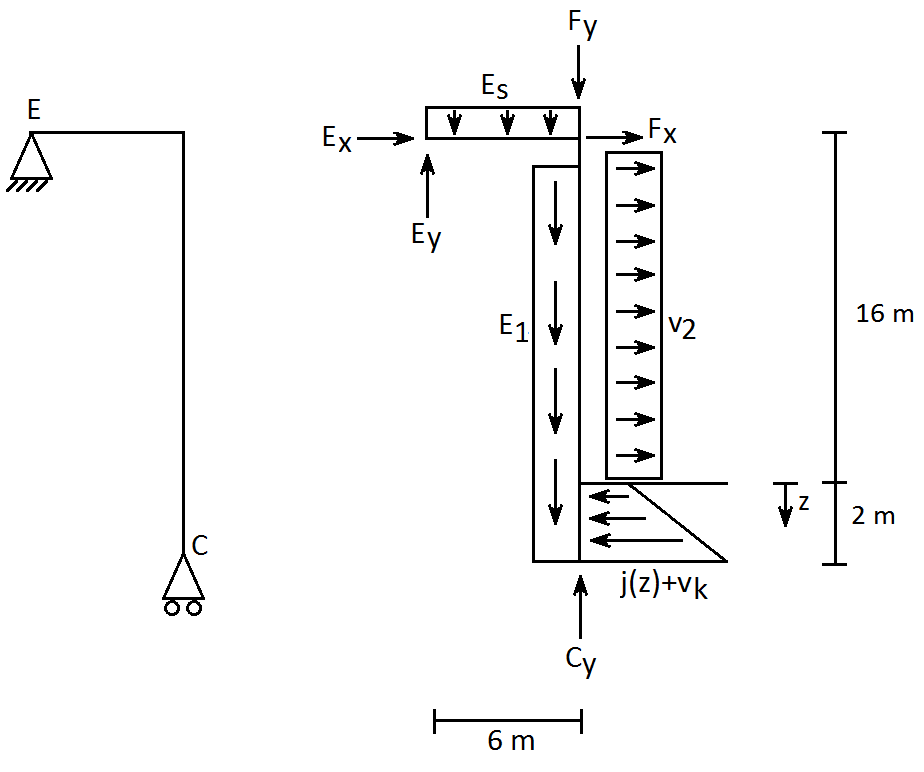
\includegraphics[width=0.7\textwidth]{billeder/hojre.png}
	\caption{Højre side af systemet, samt fritlegemediagram}
	\label{fig:opdelingh}
\end{figure}

\begin{figure}[H]
	\centering
	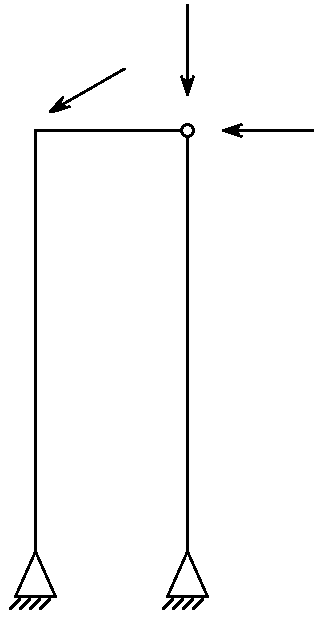
\includegraphics[width=0.7\textwidth]{billeder/venstre.png}
	\caption{Venstre side af systemet, samt fritlegemediagram}
	\label{fig:opdelingv}
\end{figure}

Reaktionerne i punkt E kan sættes som punktlaster i charnieret på den venstre side af systemet, som ses på Figur \ref{fig:opdelingv}. Reaktionerne på højre del af systemet beregnes først.
\newline
\newline
Først bestemmes den vandrette reaktion i charnieret, $E_x$ gennem vandret ligevægt: 
\begin{equation}
\begin{split}
	$$+\atop\rightarrow$$: 0 = & F_x + E_x - j - v_k \cdot \SI{2}{m} - v_2 \cdot \SI{16}{m}
	\\ &
	E_x = \SI{62,52}{kN}
\end{split}
\end{equation}

$C_y$ bestemmes gennem momentligevægt om punkt E: 
\begin{equation}
\begin{split}
	\ALN{\text{E}} :0 = & -F_y \cdot \SI{6}{m} - E_1 \cdot \SI{18}{m} \cdot \SI{6}{m} + C_y \cdot \SI{6}{m} - j \cdot \SI{17,33}{m} - v_k \cdot \SI{2}{m} \cdot \SI{17}{m} \\ & - E_s \cdot \SI{6}{m} \cdot \SI{3}{m} - v_2 \cdot \SI{16}{m} \cdot \SI{8}{m}
	\\ &
	C_y = \SI{964,68}{kN}
\end{split}
\end{equation}

Til sidst bestemmes den lodrette reaktion i charnierledet, $E_y$ gennem lodret ligevægt: 
\begin{equation}
\begin{split}
	\uparrow+: 0 = & F_y - E_1 \cdot \SI{18}{m} - E_s \cdot \SI{6}{m} + C_y + E_y
	\\ &
	E_y = \SI{-349,74}{kN}
\end{split}
\end{equation}

Reaktionerne $E_y$ og $E_x$ påsættes som belastninger i punkt E på det venstre system, så de virker som vist på Figur \ref{fig:opdelingv}. Reaktionerne i det venstre system kan hermed bestemmes.
\\
\\
Først tages der moment om A, for at beregne $B_y$:
\begin{equation}
\begin{split}
	\ALN{\text{A}}: 0 = & B_y \cdot \SI{6}{m} + E_y \cdot \SI{6}{m} + E_x \cdot \SI{18}{m} - E_2 \cdot \SI{18}{m} \cdot \SI{6}{m} - E_s \cdot \SI{6}{m} \cdot \SI{3}{m} \\ & + D_x \cdot \SI{18}{m} - v_1 \cdot \SI{16}{m} \cdot (\SI{8}{m} + \SI{2}{m}) - j \cdot (\SI{2}{m} \cdot \frac{1}{3}) - v_k \cdot \SI{2}{m} \cdot \SI{1}{m}
	\\ &
	B_y = \SI{658,26}{kN}
\end{split}
\end{equation}

Nu laves lodret ligevægt for at bestemme $A_y$:
\begin{equation}
\begin{split}
	\uparrow+: 0 = & A_y + B_y - E_y - E_2 \cdot \SI{18}{m} - E_1 \cdot \SI{18}{m} - F_y - E_s \cdot \SI{6}{m}
	\\ &
	A_y = \SI{732,77}{kN}
\end{split}
\end{equation}

For at gøre det muligt at isolere en af de vandrette reaktioner laves der et snit i charnieret. Derefter betragtes den nedre del, og der tages moment omkring charnieret i punkt E, for at bestemme $B_x$:
\begin{equation}
\begin{split}
	\ALN{\text{E}}: 0 = & B_x \cdot \SI{18}{m}
	\\ &
	B_x = \SI{0}{kN}
\end{split}
\end{equation}

Slutteligt laves vandret ligevægt for at bestemme $A_x$:
\begin{equation}
\begin{split}
	$$+\atop\rightarrow$$: 0 = & A_x - E_x + B_x + j + v_k \cdot \SI{2}{m} + v_1 \cdot \SI{16}{m} - D_x
	\\ &
	A_x = \SI{-133,31}{kN}
\end{split}
\end{equation} 

\section{Snitkræfter}
Snitkræfterne for stålrammen til tilbygningen til Strøybergs Palæs kan nu beregnes. Her laves der syv snit, som er illustreret på Figur \ref{fig:snitbrud}. Disse resultater vil bruges til at undersøge, om konstruktionen har en tilstrækkelig bæreevne, eller om den vil bryde sammen. 

\begin{figure}[H]
	\centering
	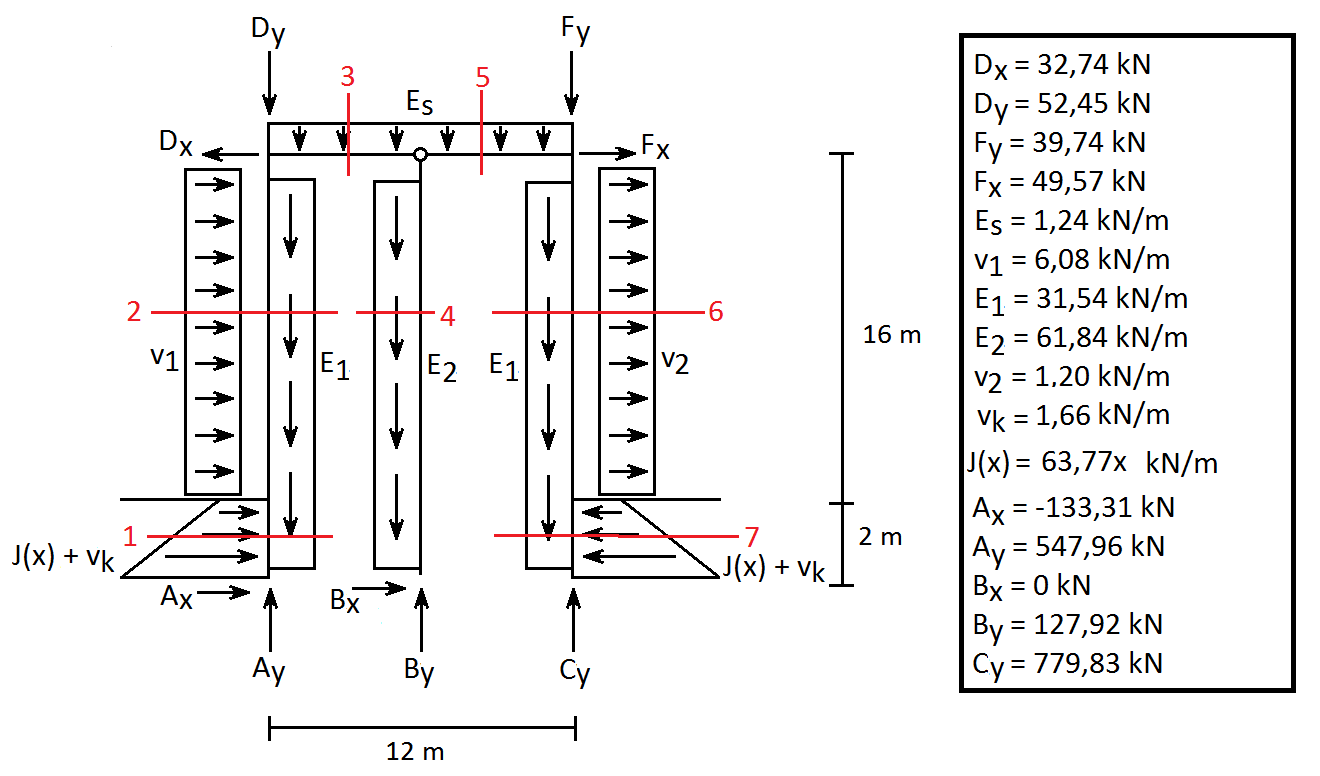
\includegraphics[width=0.8\textwidth]{billeder/snitbrud.png}
	\caption{Snit}
	\label{fig:snitbrud}
\end{figure}

Nedenfor vises beregningseksempel for snit 1 og snit 5. Beregningerne for de resterende snit kan ses i Bilag ???. 
\newline
\newline
\textbf{Snit 1: 0 m < x < 2 m}
\newline
Fritlegemediagrammet for snit 1 ses på Figur \ref{fig:snitet}.
\newline
\newline
Først bestemmes normalkraften:
\begin{equation}
	0 = N_1 + A_y - E_1 \cdot x \leftrightarrow N_1(x) = 31,\!54 \frac{\text{kN}}{\text{m}} x - \SI{547,95}{kN}
\end{equation}

Nu bestemmes forskydningskraften:
\begin{equation}
	0 = V_1 + j + v_k \cdot x + A_x \leftrightarrow V_1(x) = -33,\!64\frac{\text{kN}}{\text{m}} x + \SI{133,31}{kN}
\end{equation}

Til sidst bestemmes moment:
\begin{equation}
	0 = M_1 + j \cdot \frac{2x}{3} + v_k \cdot x \cdot \frac{x}{2} + A_x \cdot x \leftrightarrow M_1(x) = -22,\!15\frac{\text{kN}}{\text{m}} x^2 + \SI{133,30}{kN} x
\end{equation}

Alle resultater kan ses i Tabel \ref{tab:resultaterbrud}.

\begin{figure}[H]\centering
	\begin{minipage}[b]{0.48\textwidth}\centering
		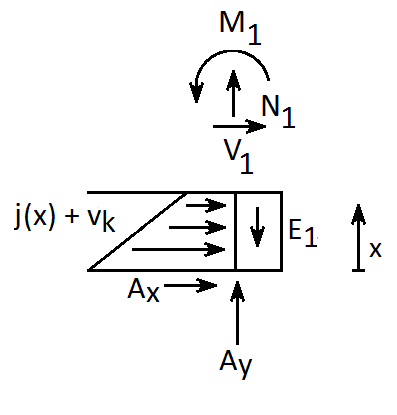
\includegraphics[width=0.80\textwidth]{billeder/snitet.png} %Venstre billede
	\end{minipage}\hfill
	\begin{minipage}[b]{0.48\textwidth}\centering
		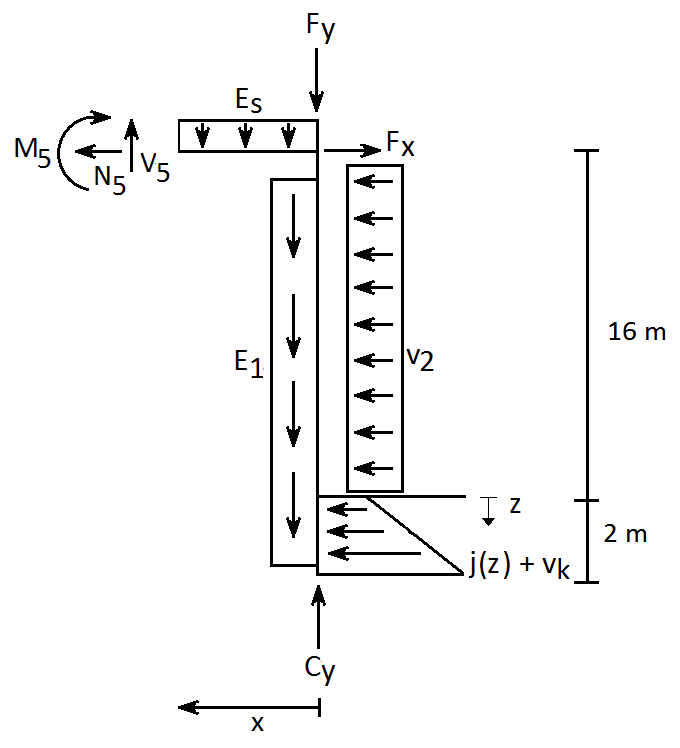
\includegraphics[width=1.0\textwidth]{billeder/snitfem.png} %Højre billede
	\end{minipage}\\ %Captions and labels
	\begin{minipage}[t]{0.48\textwidth}
		\caption{Fritlegemediagram for snit 1} %Venstre caption og label
		\label{fig:snitet}
	\end{minipage}\hfill
	\begin{minipage}[t]{0.48\textwidth}
		\caption{Fritlegemediagram for snit 5} %Højre caption og label
		\label{fig:snitfem}
	\end{minipage}
\end{figure}

\textbf{Snit 5: 0 m < x < 6 m}
\newline
Fritlegemediagrammet for snit 1 ses på Figur \ref{fig:snitfem}.
\newline
\newline
Normalkraften bestemmes først:
\begin{equation}
	0 = - N_5 + F_x - v_2 \cdot \SI{16}{m} - j - v_k \cdot 2m \leftrightarrow N_5 = \SI{49,57}{kN} - \SI{48,12}{kN} = \SI{1,45}{kN}
\end{equation}

Forskydningskraften for snit 5 bestemmes ved:
\begin{equation}
	0 = V_5 - E_1 \cdot \SI{18}{m} - F_y + C_y - E_s \cdot x \leftrightarrow V_5(x) = \SI{-172,35}{kN} + 1,\!24 \frac{\text{kN}}{\text{m}}x
\end{equation}

Til sidst bestemmes moment:
\begin{equation}
\begin{split}
	0 = & - M_5 - F_y \cdot x - E_1 \cdot \SI{18}{m} \cdot x - E_s \cdot x \frac{x}{2} - v_2 \cdot \SI{16}{m} \cdot \SI{8}{m} - v_k \cdot \SI{2}{m} \cdot \SI{17}{m} - j \cdot \SI{17,33}{m} + C_y \cdot x \leftrightarrow \\ & M_5(x) =  \SI{172,35}{kN} \cdot x - 0,\!62 \frac{\text{kN}}{\text{m}} \cdot x^2 - \SI{1011,72}{kNm}
\end{split}
\end{equation}

Tabel \ref{tab:resultaterbrud} viser resultaterne for alle snittene, som bruges til at beregne spændingstilstanden. 

\begin{table}
	\begin{center}
		\begin{tabular}{|c|c|c|c|c|c|c|}
			\hline
			Snit/Værdi & N($x_{min}$) & N($x_{max}$) & V($x_{min}$) & V($x_{max}$) & M($x_{min}$) & M($x_{max}$) 	\\ \hline
			1, 0<x<2  & -547,95       & -484,87    	&  133,31    	&  66,02 	&  0,00     &  178.00        		\\ \hline
			2, 2<x<18 &  -484,87        &  19,78       &  53,85      & -43,46   &  178,00  &  455,80    \\ \hline
			3, 0<x<6  & 1,45       &  1,45     &  -72,24         &  -79,69     &  403,78     &  0,21 			    \\ \hline
			4, 0<x<18 &  -1027,92       &  85,20      &  0,00        &  0,00    &  0,00   &   0,00    \\ \hline
			5, 0<x<6  &  1,45     &    1,45      &  -172,35      &  -164,89     &   -1011,72        &   0,00      		\\ \hline
			6, 2<x<18 &  -716,74  &   -212,09  &   -64,89    &   -45,73    &    -88,62       &   -1011,94      		\\ \hline
			7, 0<x<2 &  -779,83        &   -716,75       &     0,00      &   -67,29   &    0,00     &    -88,62     		\\ \hline
		\end{tabular}
		\caption{Snitkræfter for brudgrænsetilstand, N og V: kN og M: $kNm$}
		\label{tab:resultaterbrud}
	\end{center}
\end{table}

Ud fra snittene er der lavet snitkurver, som er illusteret på Figur \ref{fig:forskydningskurve}, Figur \ref{fig:momentkurve} og Figur \ref{fig:normalkraftkurve}. Værdierne i kurverne aflæses i Tabel \ref{tab:resultaterbrud}, hvor $V_1$ angiver værdien for forskydningskraften ved snit 1. Altså er $V_1(0m) = 133,31 kN$, $V_1(2m) = 66,02 kN$, osv.

\begin{figure}[H]
	\centering
	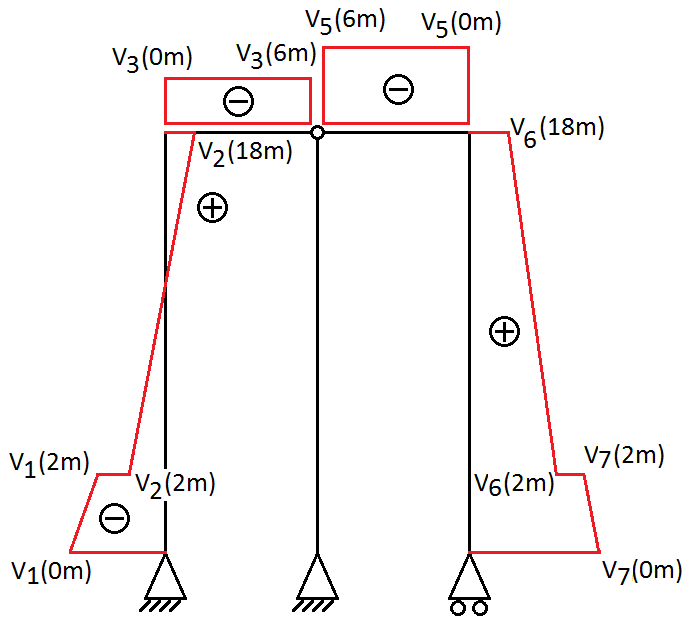
\includegraphics[width=0.7\textwidth]{billeder/sk.png}
	\caption{Forskydningskurve}
	\label{fig:forskydningskurve}
\end{figure}

\begin{figure}[H]
	\centering
	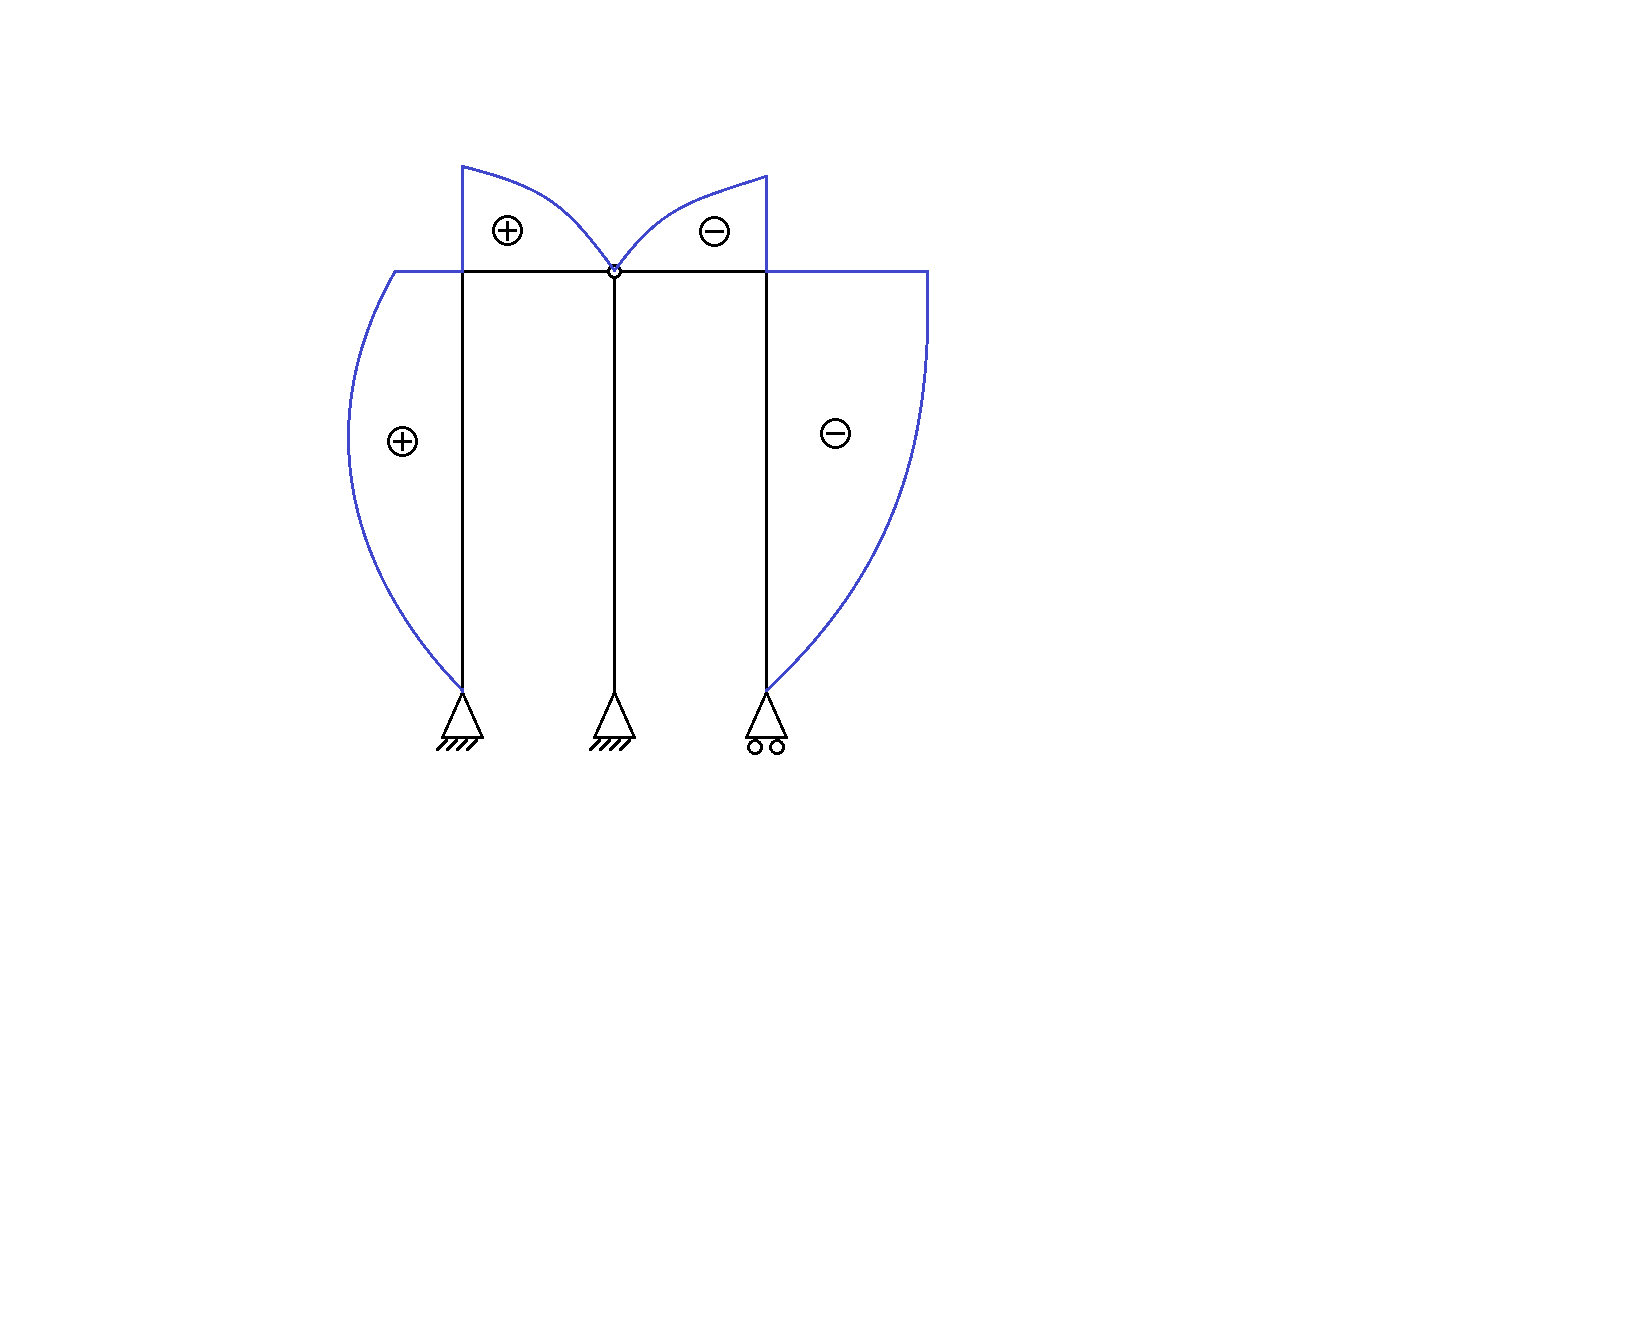
\includegraphics[width=0.7\textwidth]{billeder/skkm.png}
	\caption{Momentkurve}
	\label{fig:momentkurve}
\end{figure}

\begin{figure}[H]
	\centering
	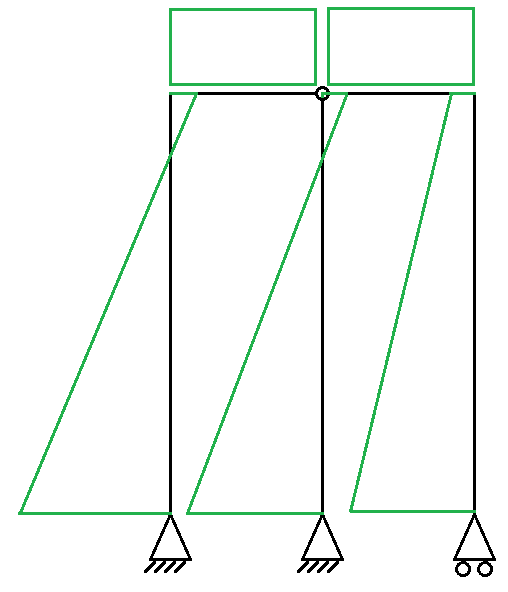
\includegraphics[width=0.7\textwidth]{billeder/SKFN.png}
	\caption{Normalkraftkurve}
	\label{fig:normalkraftkurve}
\end{figure}

\section{Spænding}

\begin{figure}[H]
	\centering
	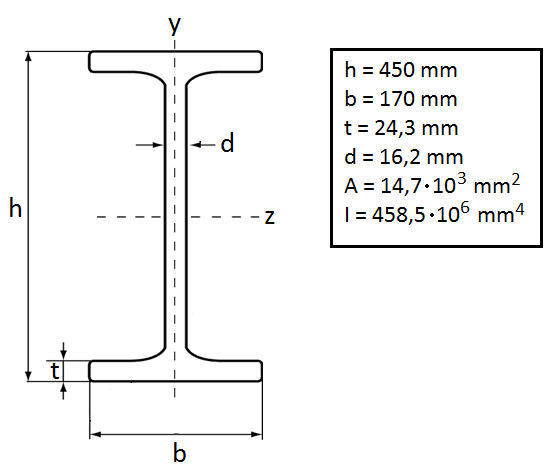
\includegraphics[width=0.4\textwidth]{billeder/iprofil.png}
	\caption{I-profil 450}
	\label{fig:iprofil}
\end{figure}

Hovedformålet med dette afsnit, er at finde ud af om konstruktionen har en tilstrækkelig bæreevne. Derfor undersøges spændingstilstanden ved: 
\begin{equation}
\sqrt{\sigma^2 + 3\tau^2} \le \frac{f_{yk}}{\gamma}
\end{equation}

\begin{itemize}
	\item[-] $\sigma$: Normalspænding 
	\item[-] $\tau$: Forskydningsspænding
	\item[-] $f_{yk}$: Den karakteristiske flydespænding, der afhænger af ståltype. For ståltype S235 ved $16 < t \le 40$ er $f_{yk} = 225 MPa$ \citep[ s. 213]{stabi}
	\item[-] $\gamma$: Partialkoefficient, der sættes til 1,1 \citep[ s. 212]{stabi}.
\end{itemize}

Spændingstilstanden undersøges i tre forskellige snit på I-profilet, som ses på Figur \ref{fig:iprofilsnit}.

\begin{figure}[H]
	\centering
	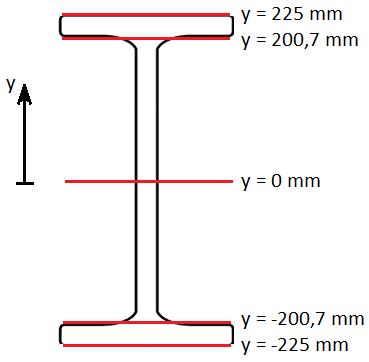
\includegraphics[width=0.4\textwidth]{billeder/iprofilsnit.png}
	\caption{I-profil med snit}
	\label{fig:iprofilsnit}
\end{figure}

Først skal normal- og forskydningsspændingen beregnes, som gøres nedenfor. 

\subsection{Forskydningsspænding}
SKRIV KORT HVAD FORSKYDNINGSSPÆNDING ER.
\newline
Forskydningsspændingen $\tau$ beregnes ved Grasshofs formel:

\begin{equation}
\tau = \frac{VQ}{Ib}
\end{equation}

\begin{itemize}
	\item[-] V: Forskydningskraft, som er bestemt igennem snitkræfter
	\item[-] Q: Statisk moment
	\item[-] b: Bredde
\end{itemize}

Forskydningsspændingsfordelingen på I-profilet findes ved, at lave to snit på I-profilet, som er illustreret på Figur \ref{fig:snitsnit}. 

\begin{figure}[H]
	\centering
	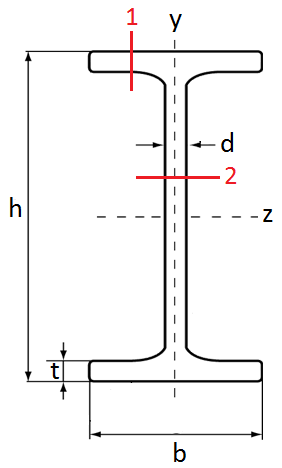
\includegraphics[width=0.4\textwidth]{billeder/forskydningprofil.png}
	\caption{BILLETEKST}
	\label{fig:snitsnit}
\end{figure}

Den ubekendte faktor til beregningen af forskydningsspændingen er det statiske moment \textit{Q}, der er defineret som:
\begin{equation}
Q = \bar{y}A
\end{equation}
\begin{itemize}
	\item[-] $\bar{y}$: Tyngdepunktskoordinat
	\item[-] A: Areal
\end{itemize}

Q beregnes for henholdsvis snit 1 og snit 2, hvormed forskydningsspændingen kan beregnes. 
\newline
\newline
\textbf{Snit 1: Forskydningsspændingsfordeling i flangen}
\newline
Snit 1 er vist på Figur \ref{fig:snitetforskyd}, hvor 0 mm < z < 76,9 mm

\begin{figure}[H]
	\centering
	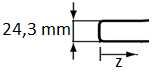
\includegraphics[width=0.4\textwidth]{billeder/snitetforskydning.png}
	\caption{Snit 1}
	\label{fig:snitetforskyd}
\end{figure}

Tyngdepunktskoordinat $\bar{y}$ samt arealet bestemmes:
\begin{equation}
\bar{y} = \frac{450 \text{mm} - 2 \cdot 24,\!3 \textbf{mm}}{2} + \frac{24,\!3 \text{mm}}{2} = 212,\!85 \text{mm}
\end{equation}
\begin{equation}
A = z \cdot \SI{24,3}{mm}
\end{equation}

Dermed bestemmes det statiske moment til:
\begin{equation}
Q(z) = \SI{212,85}{mm} \cdot (z \cdot \SI{24,3}{mm})
\end{equation}

z sættes til 0 mm og 76,9 mm for at kunne bestemmes den mindste og største forskydningsspænding:
\begin{equation}
Q_0 = \SI{212,85}{mm} \cdot (\SI{0}{mm} \cdot \SI{24,3}{mm}) = \SI{0}{mm^3}
\end{equation} 
\begin{equation}
Q_{76,9} = \SI{212,85}{mm} \cdot (\SI{76,9}{mm} \cdot \SI{24,3}{mm}) = \SI{3,977 \cdot 10^5}{mm^3}
\end{equation}

Dermed kan den mindste og den største forskydningsspænding bestemmes, hvor kun V afhænger af hvilket snit på konstruktionen der vælges:
\begin{equation}
\tau_{max} = \frac{V \cdot 3,977 \cdot 10^5 \text{mm^3}}{458,\!5 \cdot 10^6 \text{mm^4} \cdot 24,\!3 \text{mm}}
\end{equation}

\begin{equation}
\tau_{min} = \frac{V \cdot 0 \text{mm^3}}{458,\!5 \cdot 10^6 \text{mm^4} \cdot 24,\!3 \text{mm}} = 0 MPa
\end{equation}

INDSÆT TABEL MED RESULTATER FOR DE VALGTE SNIT SAMT FIGUR OVER HVORDAN FORSKYDNINGSSPÆNDINGEN FORDELER SIG I FLANGEN

\begin{figure}[H]
	\centering
	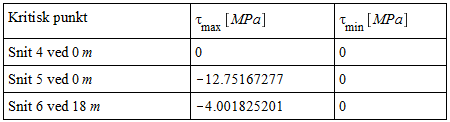
\includegraphics[width=0.4\textwidth]{billeder/tabelsnitet.png}
	\caption{TABEL SKAL LAVES PÆNT}
	\label{fig:tabeltabeltab}
\end{figure}

\begin{figure}[H]
	\centering
	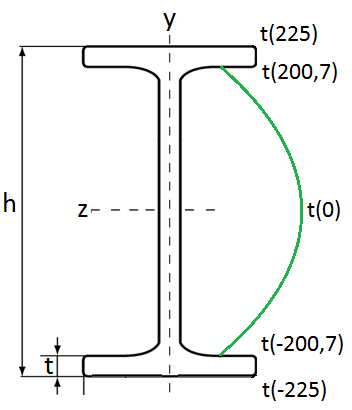
\includegraphics[width=0.4\textwidth]{billeder/forskydningsfordeling.png}
	\caption{Forskydningsspændingsfordeling}
	\label{fig:fordeling}
\end{figure}

\textbf{Snit 2: Forskydningsspændingsfordeling i kroppen}
\newline
Snit 2 er vist på Figur \ref{fig:snittoforskyd}. 

\begin{figure}[H]
	\centering
	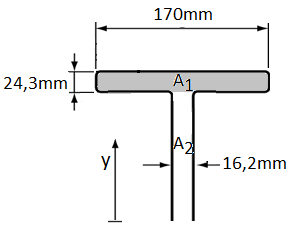
\includegraphics[width=0.4\textwidth]{billeder/snittoforskydning.png}
	\caption{Snit 2}
	\label{fig:snittoforskyd}
\end{figure}

Som det ses på Figur \ref{fig:snittoforskyd} er I-profilet inddelt i to arealer; $A_1$ og $A_2$. Derfor findes en Q for hver areal; $Q_1$ og $Q_2$, og den samlede Q er dermed $Q = Q_1 + Q_2$. 

Først findes Q for $A_1$:
\begin{equation}
Q_1 = \SI{24,3}{mm} \cdot \SI{170}{mm} \cdot (\SI{225}{mm} - \frac{1}{2} \cdot \SI{24,3}{mm}) = \SI{8,793 \cdot 10^5}{mm^3}
\end{equation}

$Q_1$ er altså en konstant, idet den ikke er afhængig af y.
\newline
\newline
Q for $A_2$, som er afhængig af y, bestemmes nu:
\begin{equation}
Q_2(y) = (\SI{16,2}{mm} \cdot (\SI{200,7}{mm} -y)) \cdot (\frac{200\!,7 \text{mm} -y}{2} + y)
\end{equation}

Hermed fås en samlet Q som funktion af y:
\begin{equation}
Q(y) = \SI{8,793 \cdot 10^5}{mm^3} + ((\SI{16,2}{mm} \cdot (\SI{200,7}{mm} -y)) \cdot (\frac{200\!,7 \text{mm} -y}{2} + y))
\end{equation}

Forskydningsspændingen kan hermed beregnes ved:
\begin{equation}
\tau(y) = \frac{V Q(y)}{458,\!5 \cdot 10^6 \text{mm^4} \cdot 16,\!2 \text{mm}}
\end{equation}

Ved at sætte y til 0 og $\pm 200,7 mm$ findes forskydningsspændingerne langs I-profilet krop. Forskydningsspændingen vil altid være 0 i oversiden, dvs. ved y = 225 mm. Forskydningsspændingsfordeling er illustreret på Figur \ref{fig:forskydfordeling}. Resultatet af forskydningsspændingsfordeling ses i Tabel XXX.  

\begin{figure}[H]
	\centering
	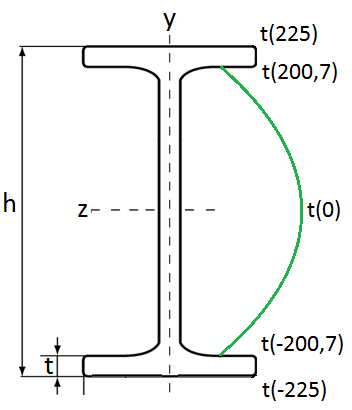
\includegraphics[width=0.4\textwidth]{billeder/forskydningsfordeling.png}
	\caption{Forskydningsspændingsfordeling}
	\label{fig:forskydfordeling}
\end{figure}

\subsection{Normalspænding}
SKRIV KORT HVAD NORMALSPÆNDING ER.
\newline
Normalspændingen $\sigma$ findes ved Naviers formel:
\begin{equation}
\sigma = \frac{N}{A} - \frac{M}{I} y
\end{equation}

\begin{itemize}
	\item[-] N: Normalkraft, som er bestemt igennem snitkræfter
	\item[-] A: Tværsnitsareal, som for stålprofil 450 er $14,\!7 \cdot 10^3 mm^2$ \citep{stabi}. 
	\item[-] M: Moment, som er bestemt igennem snitkræfter
	\item[-] y: Koordinat til snit
	\item[-] I: Inertimoment, som for stålprofil 450 er $458,\!5 \cdot 10^6 mm^4$ \citep{stabi}. 
\end{itemize} 

Her er den eneste ubekendte faktor y. Derfor fås normalspændingen som en funktion af y, hvor N og M varierer efter hvilket snit på konstruktionen der undersøges:
\begin{equation}
\sigma(y) = \frac{N}{14,\!7 \cdot 10^3 \text{mm^2}} - \frac{M}{458,\!5 \cdot 10^6 \text{mm^4}} y
\end{equation}
Spændingen beregnes, ligesom forskydningskraften, til $y = 0 mm$, $y = \pm 200,\!7 mm$ og $y = \pm 225 mm$. Resultatet ses i tabel XXX. 

\subsection{Spændingstilstand}
Den regningsmæssige flydespænding $f_y$ bestemmes til:
\begin{equation}
f_y = \frac{225 \text{MPa}}{1,\!1} = 204,\!54 MPa
\end{equation}

\begin{figure}[H]
	\centering
	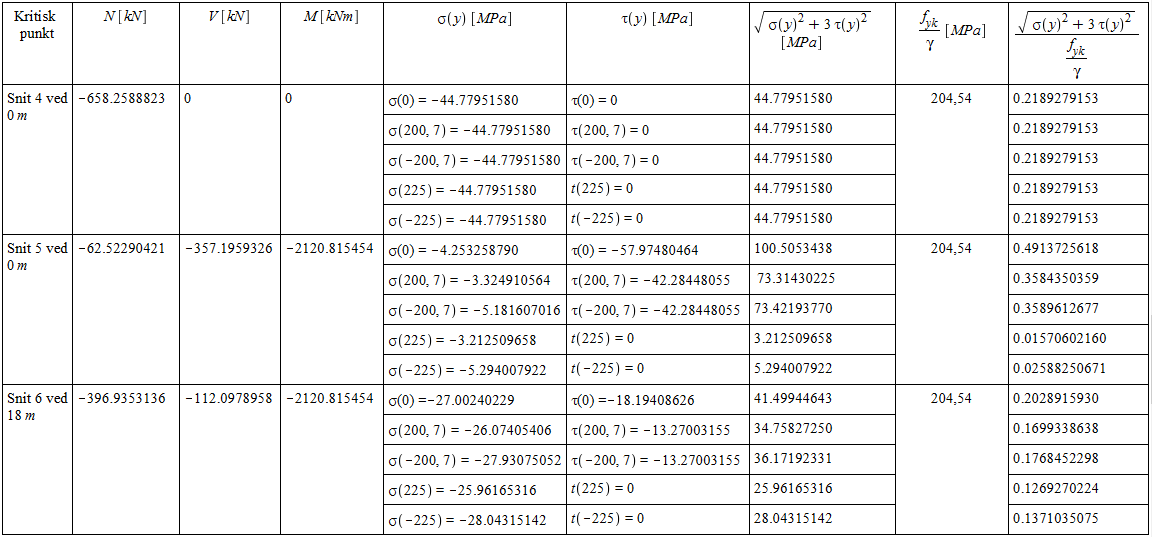
\includegraphics[width=0.4\textwidth]{billeder/tabelsnitto.png}
	\caption{TABEL SKAL LAVES PÆNT}
	\label{fig:tabeltabel}
\end{figure}
